\section{FlashAttention-2}
\begin{frame}{}
    \LARGE \textbf{FlashAttention-2}
\end{frame}


\begin{frame}{FlashAttention-2: Overview}
    \begin{itemize}
        \item \textbf{Paper:} Dao et al. (2023)
        \item \textbf{Goal:} Memory-efficient and fast attention computation
        \item \textbf{Highlights:}
        \begin{itemize}
            \item 90--95\% GPU utilization
            \item 2--4$\times$ faster than standard attention
        \end{itemize}
        \item \textbf{Techniques:}
        \begin{itemize}
            \item Multi-query and grouped-query attention
            \item Hardware-aware scheduling
            \item Supports long context windows (32k+ tokens)
        \end{itemize}
        \item \textbf{Adoption:}
        \begin{itemize}
            \item Used in OpenAI GPT-4, Mistral, LLaMA 3
            \item Critical for scaling to trillion-parameter models efficiently
        \end{itemize}
    \end{itemize}
\end{frame}


\begin{frame}[allowframebreaks]{FlashAttention-2: Key Improvements}
    \begin{itemize}
        \item \textbf{Fewer non-matmul FLOPs:}
        \begin{itemize}
            \item Algorithm tweaks reduce non-matmul operations (e.g., rescaling, masking).
            \item Maximizes use of specialized GPU units (Tensor Cores).
            \item Non-matmul FLOPs are up to 16$\times$ more expensive than matmul FLOPs.
        \end{itemize}
        \item \textbf{Better Parallelism:}
        \begin{itemize}
            \item Parallelizes over sequence length in addition to batch size and heads.
            \item Improves GPU utilization for long sequences and small batches.
        \end{itemize}
    \framebreak
        \item \textbf{Improved Work Partitioning:}
        \begin{itemize}
            \item Splits Q across warps (instead of K/V), reducing shared memory communication.
            \item Yields significant speedup by minimizing synchronization.
        \end{itemize}
        \item \textbf{New Features:}
        \begin{itemize}
            \item Supports head dimensions up to 256.
            \item Enables multi-query and grouped-query attention.
        \end{itemize}
    \end{itemize}
\end{frame}

\begin{frame}[allowframebreaks]{FlashAttention-2: Architecture}
    \begin{figure}
        \centering
        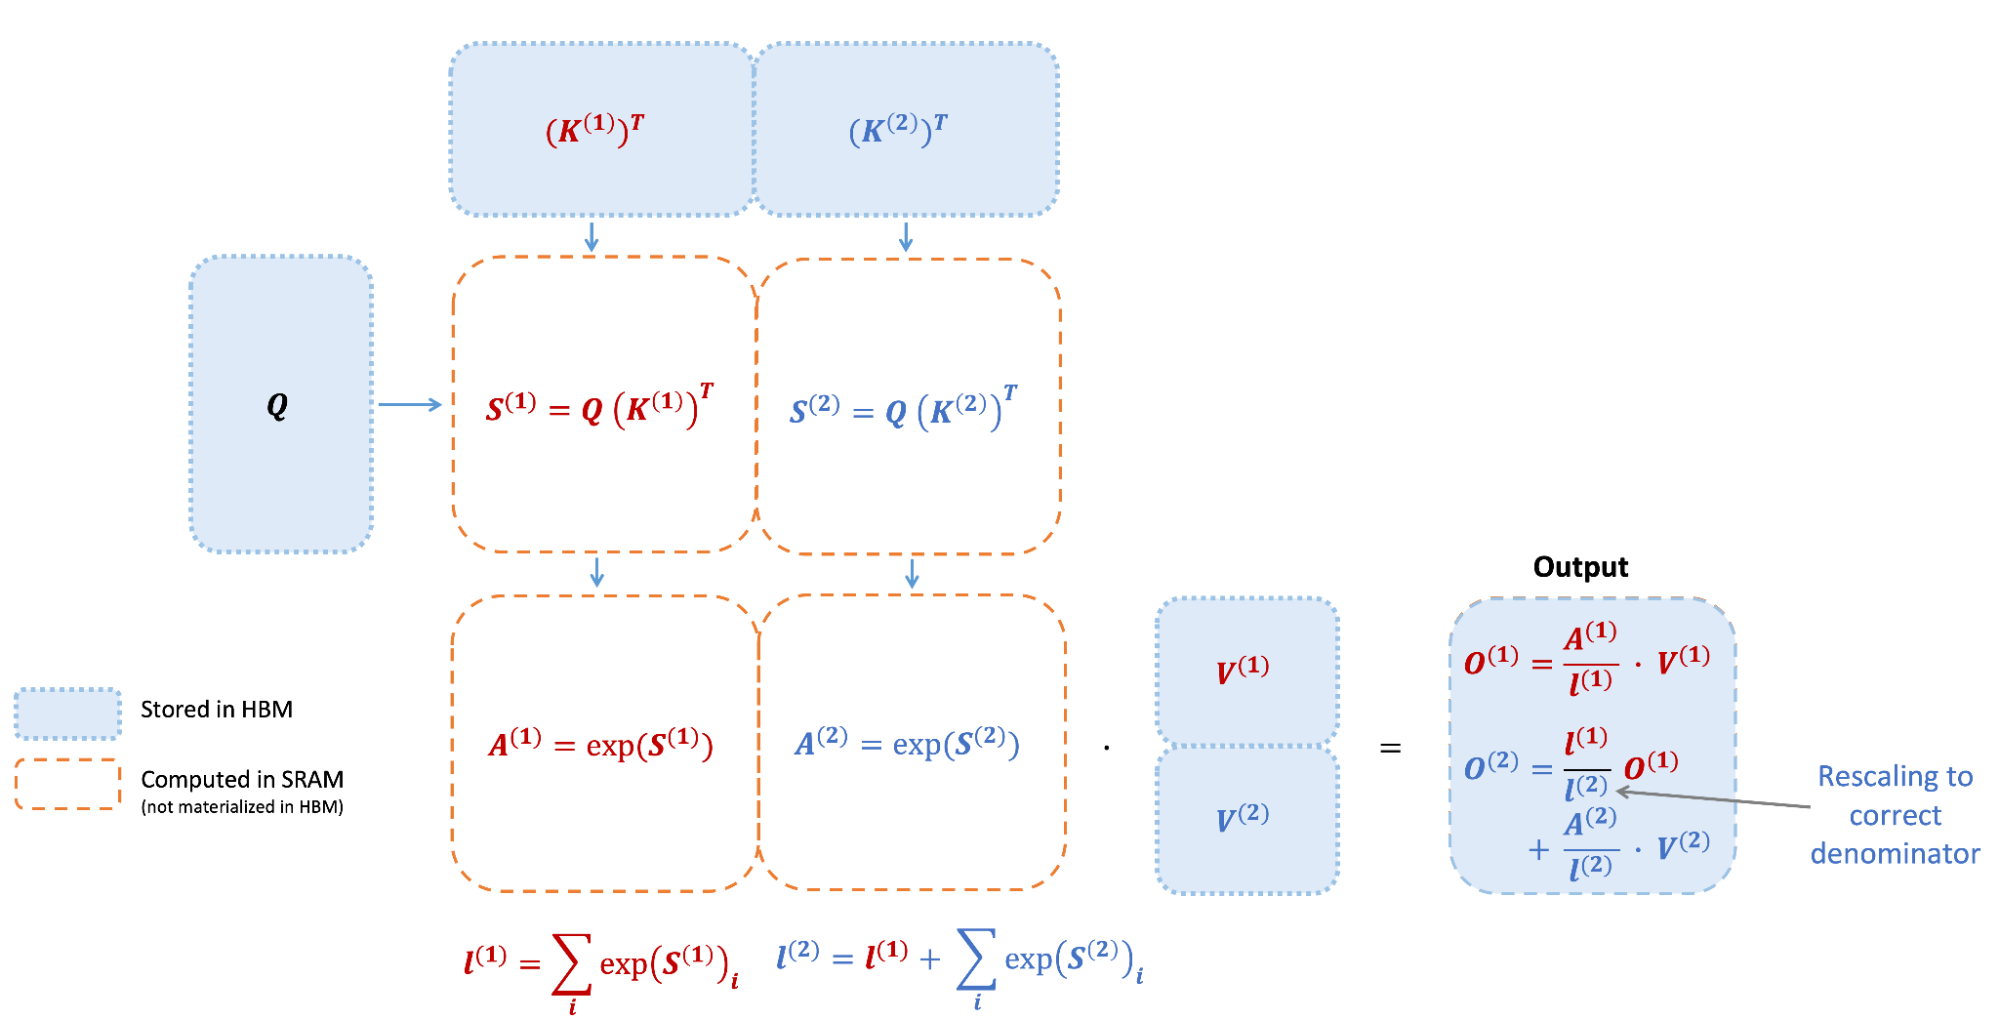
\includegraphics[height=0.88\textheight,width=1.08\textwidth,keepaspectratio]{images/recent-advance/flash-attention-2-arch.png}
    \end{figure}
\framebreak
    \begin{figure}
        \centering
        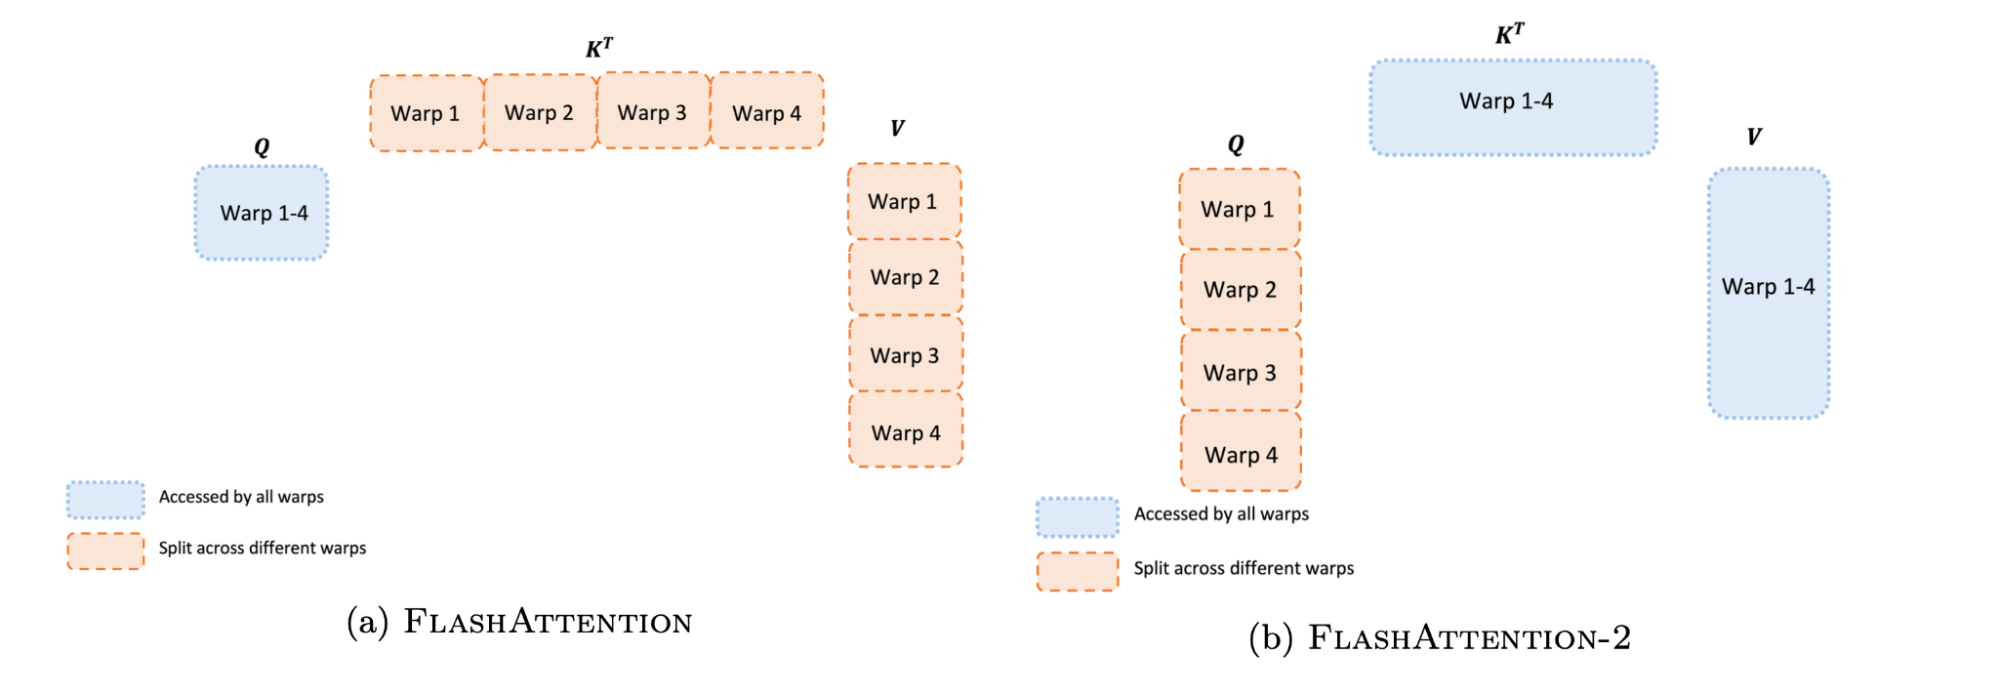
\includegraphics[height=0.88\textheight,width=1.08\textwidth,keepaspectratio]{images/recent-advance/flash-attention-2.png}
    \end{figure}
\framebreak
    \begin{itemize}
        \item \textbf{Multi-Query Attention:} Uses a single set of keys and values for all queries, reducing memory usage.
        \item \textbf{Grouped-Query Attention:} Groups queries to share keys and values, further optimizing memory.
        \item \textbf{Hardware-Aware Scheduling:} Optimizes GPU scheduling to maximize throughput and minimize latency.
        \item \textbf{Long Context Support:} Efficiently handles long sequences (32k+ tokens) with minimal memory overhead.
    \end{itemize}
\framebreak
    \begin{figure}
        \centering
        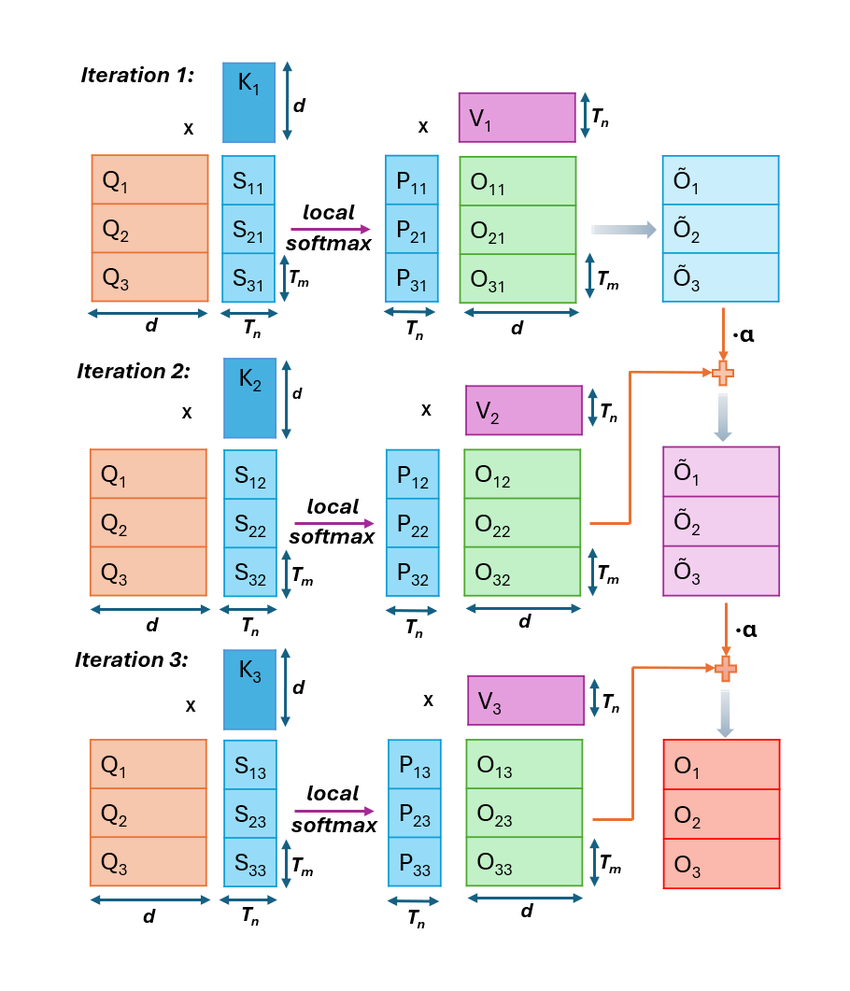
\includegraphics[height=0.82\textheight,width=\textwidth,keepaspectratio]{images/recent-advance/flash-attention-2-iterative-update.png}
        \caption*{Iterative update of output in FlashAttention-2 with Cn = 3 iterations.}
    \end{figure}
\end{frame}

\begin{frame}{FlashAttention-2: Performance Benchmarks}
    \begin{itemize}
        \item \textbf{Speed:}
        \begin{itemize}
            \item Up to 2$\times$ faster than FlashAttention-1, 9$\times$ faster than standard PyTorch attention.
            \item Achieves up to 335 TFLOPs/s on H100 GPUs.
        \end{itemize}
        \item \textbf{End-to-End Training:}
        \begin{itemize}
            \item 1.3$\times$ speedup over optimized FlashAttention models.
            \item Up to 225 TFLOPs/s on A100 GPU (72\% model FLOPs utilization).
        \end{itemize}
        \item \textbf{Example Results:}
            \begin{tabular}{lccc}
                \toprule
                Model & Baseline & FlashAttention & FlashAttention-2 \\
                \midrule
                GPT3-1.3B 2k & 142 & 189 & 196 \\
                GPT3-1.3B 8k & 72 & 170 & 220 \\
                GPT3-2.7B 2k & 149 & 189 & 205 \\
                GPT3-2.7B 8k & 80 & 175 & 225 \\
                \bottomrule
            \end{tabular}
        \item \footnotesize{Baseline: Megatron-LM without FlashAttention.}
    \end{itemize}
\end{frame}